\documentclass[14pt]{extbook}
\usepackage{multicol, enumerate, enumitem, hyperref, color, soul, setspace, parskip, fancyhdr} %General Packages
\usepackage{amssymb, amsthm, amsmath, bbm, latexsym, units, mathtools} %Math Packages
\everymath{\displaystyle} %All math in Display Style
% Packages with additional options
\usepackage[headsep=0.5cm,headheight=12pt, left=1 in,right= 1 in,top= 1 in,bottom= 1 in]{geometry}
\usepackage[usenames,dvipsnames]{xcolor}
\usepackage{dashrule}  % Package to use the command below to create lines between items
\newcommand{\litem}[1]{\item#1\hspace*{-1cm}\rule{\textwidth}{0.4pt}}
\pagestyle{fancy}
\lhead{Makeup Progress Quiz 3}
\chead{}
\rhead{Version B}
\lfoot{4315-3397}
\cfoot{}
\rfoot{Fall 2020}
\begin{document}

\begin{enumerate}
\litem{
Solve the rational equation below. Then, choose the interval(s) that the solution(s) belongs to.\[ \frac{-30}{-30x -30} + 1 = \frac{-30}{-30x -30} \]\begin{enumerate}[label=\Alph*.]
\item \( x \in [-3.0,0.0] \)
\item \( \text{All solutions lead to invalid or complex values in the equation.} \)
\item \( x_1 \in [-2, 0] \text{ and } x_2 \in [1,4] \)
\item \( x_1 \in [-2, 0] \text{ and } x_2 \in [-1,0] \)
\item \( x \in [0,3] \)

\end{enumerate} }
\litem{
Solve the rational equation below. Then, choose the interval(s) that the solution(s) belongs to.\[ \frac{2x}{6x + 3} + \frac{-6x^{2}}{30x^{2} +27 x + 6} = \frac{2}{5x + 2} \]\begin{enumerate}[label=\Alph*.]
\item \( x_1 \in [-1.15, -0.42] \text{ and } x_2 \in [-0.2,3.8] \)
\item \( \text{All solutions lead to invalid or complex values in the equation.} \)
\item \( x_1 \in [-1.15, -0.42] \text{ and } x_2 \in [-0.9,0.7] \)
\item \( x \in [-0.53,-0.17] \)
\item \( x \in [2.2,2.73] \)

\end{enumerate} }
\litem{
Choose the graph of the equation below.\[ f(x) = \frac{-1}{x + 3} - 3 \]\begin{enumerate}[label=\Alph*.]
\begin{multicols}{2}\item 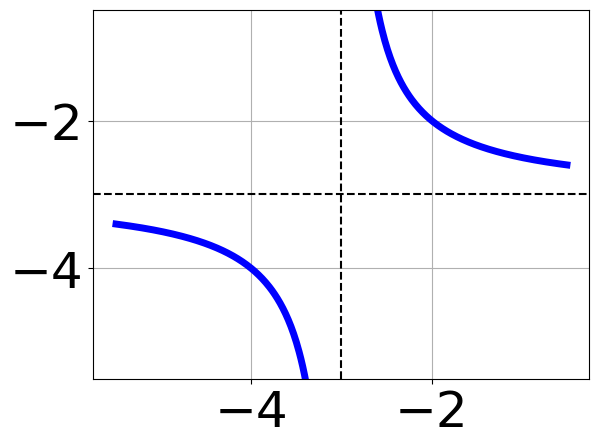
\includegraphics[width = 0.3\textwidth]{../Figures/rationalEquationToGraphCopyAB.png}\item 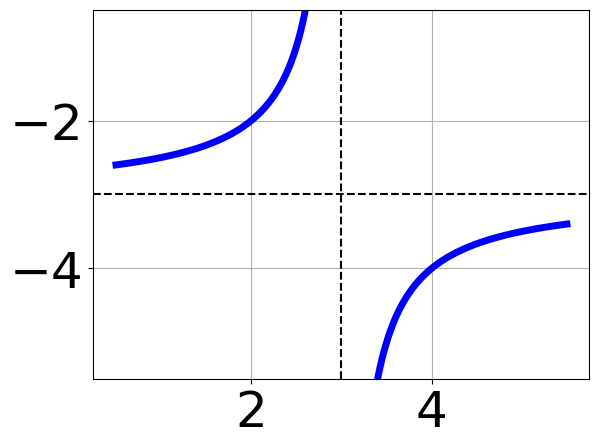
\includegraphics[width = 0.3\textwidth]{../Figures/rationalEquationToGraphCopyBB.png}\item 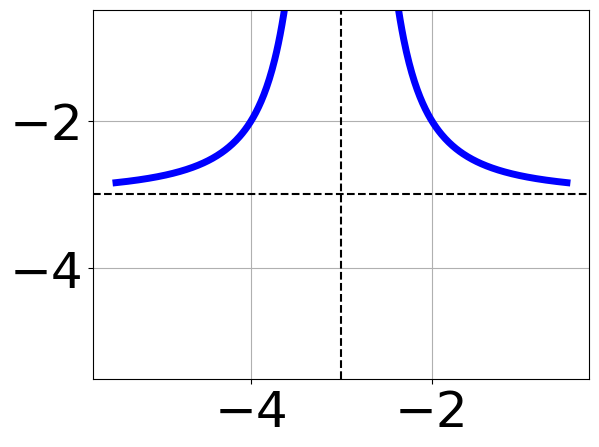
\includegraphics[width = 0.3\textwidth]{../Figures/rationalEquationToGraphCopyCB.png}\item 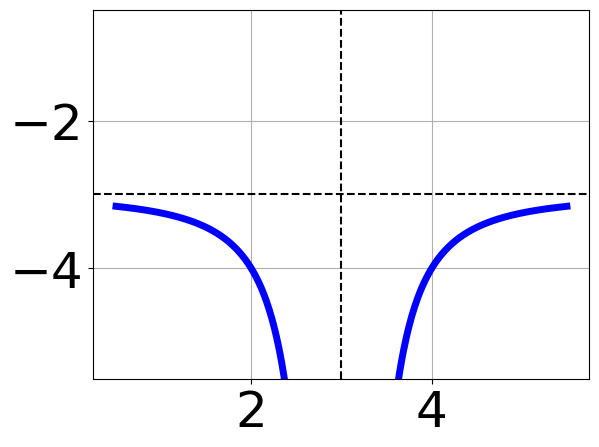
\includegraphics[width = 0.3\textwidth]{../Figures/rationalEquationToGraphCopyDB.png}\end{multicols}\item None of the above.
\end{enumerate} }
\litem{
Determine the domain of the function below.\[ f(x) = \frac{4}{30x^{2} -6 x -36} \]\begin{enumerate}[label=\Alph*.]
\item \( \text{All Real numbers except } x = a \text{ and } x = b, \text{ where } a \in [-4, 0] \text{ and } b \in [0.2, 5.2] \)
\item \( \text{All Real numbers except } x = a, \text{ where } a \in [-4, 0] \)
\item \( \text{All Real numbers except } x = a \text{ and } x = b, \text{ where } a \in [-38, -35] \text{ and } b \in [30, 31] \)
\item \( \text{All Real numbers except } x = a, \text{ where } a \in [-38, -35] \)
\item \( \text{All Real numbers.} \)

\end{enumerate} }
\litem{
Choose the equation of the function graphed below.
\begin{center}
    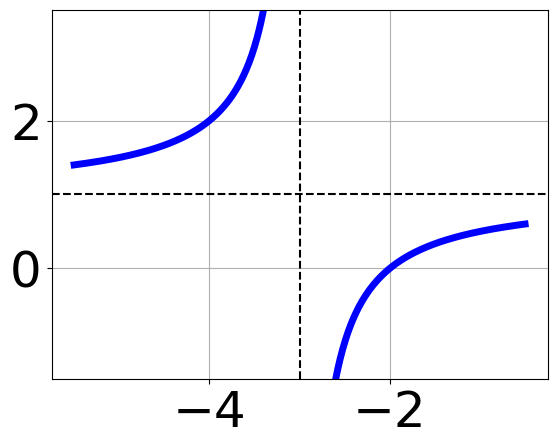
\includegraphics[width=0.5\textwidth]{../Figures/rationalGraphToEquationB.png}
\end{center}
\begin{enumerate}[label=\Alph*.]
\item \( f(x) = \frac{-1}{(x + 3)^2} + 1 \)
\item \( f(x) = \frac{-1}{x + 3} + 1 \)
\item \( f(x) = \frac{1}{x - 3} + 1 \)
\item \( f(x) = \frac{1}{(x - 3)^2} + 1 \)
\item \( \text{None of the above} \)

\end{enumerate} }
\litem{
Determine the domain of the function below.\[ f(x) = \frac{4}{15x^{2} -15} \]\begin{enumerate}[label=\Alph*.]
\item \( \text{All Real numbers.} \)
\item \( \text{All Real numbers except } x = a \text{ and } x = b, \text{ where } a \in [-10.5, -7.3] \text{ and } b \in [22.6, 25.5] \)
\item \( \text{All Real numbers except } x = a, \text{ where } a \in [-2.3, 0.4] \)
\item \( \text{All Real numbers except } x = a, \text{ where } a \in [-10.5, -7.3] \)
\item \( \text{All Real numbers except } x = a \text{ and } x = b, \text{ where } a \in [-2.3, 0.4] \text{ and } b \in [-0.4, 2.1] \)

\end{enumerate} }
\litem{
Solve the rational equation below. Then, choose the interval(s) that the solution(s) belongs to.\[ \frac{-5x}{-2x -7} + \frac{-5x^{2}}{8x^{2} +32 x + 14} = \frac{-5}{-4x -2} \]\begin{enumerate}[label=\Alph*.]
\item \( x_1 \in [-2.3, -1.1] \text{ and } x_2 \in [-1.47,3.53] \)
\item \( x_1 \in [-2.3, -1.1] \text{ and } x_2 \in [-4.5,0.5] \)
\item \( x \in [-0.6,-0.3] \)
\item \( x \in [1.2,2] \)
\item \( \text{All solutions lead to invalid or complex values in the equation.} \)

\end{enumerate} }
\litem{
Solve the rational equation below. Then, choose the interval(s) that the solution(s) belongs to.\[ \frac{-8}{4x + 2} + -9 = \frac{-3}{16x + 8} \]\begin{enumerate}[label=\Alph*.]
\item \( x \in [-0.7,0.4] \)
\item \( \text{All solutions lead to invalid or complex values in the equation.} \)
\item \( x_1 \in [-1, -0.1] \text{ and } x_2 \in [-0.4,1.8] \)
\item \( x \in [-1.7,0.3] \)
\item \( x_1 \in [-1, -0.1] \text{ and } x_2 \in [-1.8,-0.1] \)

\end{enumerate} }
\litem{
Choose the equation of the function graphed below.
\begin{center}
    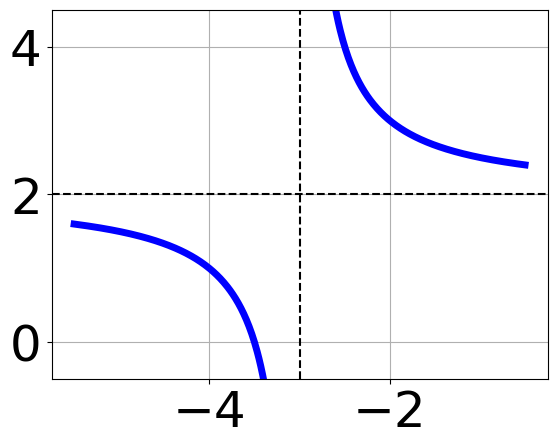
\includegraphics[width=0.5\textwidth]{../Figures/rationalGraphToEquationCopyB.png}
\end{center}
\begin{enumerate}[label=\Alph*.]
\item \( f(x) = \frac{-1}{(x - 3)^2} + 2 \)
\item \( f(x) = \frac{1}{(x + 3)^2} + 2 \)
\item \( f(x) = \frac{-1}{x - 3} + 2 \)
\item \( f(x) = \frac{1}{x + 3} + 2 \)
\item \( \text{None of the above} \)

\end{enumerate} }
\litem{
Choose the graph of the equation below.\[ f(x) = \frac{1}{x - 1} + 3 \]\begin{enumerate}[label=\Alph*.]
\begin{multicols}{2}\item 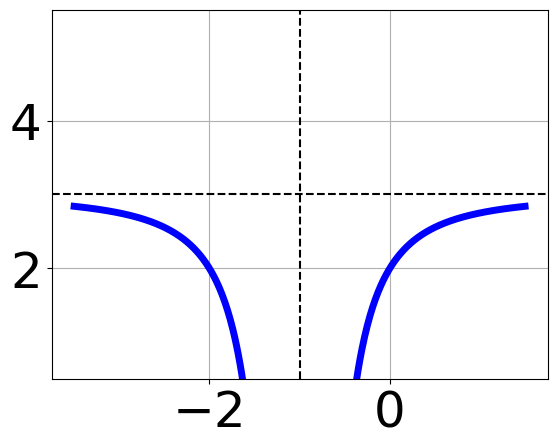
\includegraphics[width = 0.3\textwidth]{../Figures/rationalEquationToGraphAB.png}\item 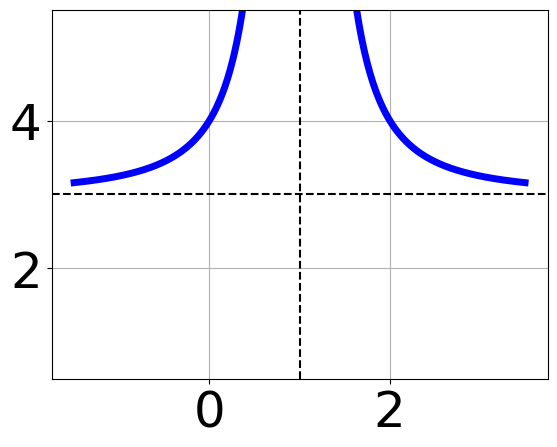
\includegraphics[width = 0.3\textwidth]{../Figures/rationalEquationToGraphBB.png}\item 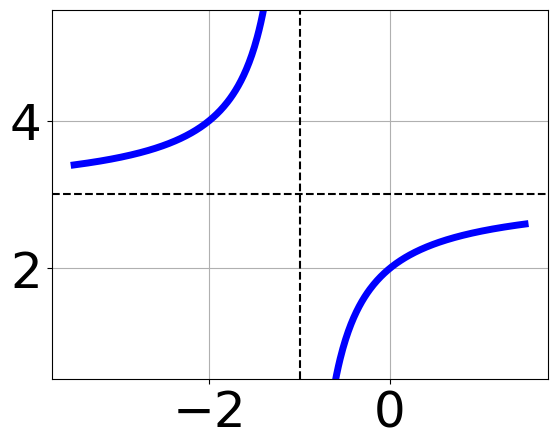
\includegraphics[width = 0.3\textwidth]{../Figures/rationalEquationToGraphCB.png}\item 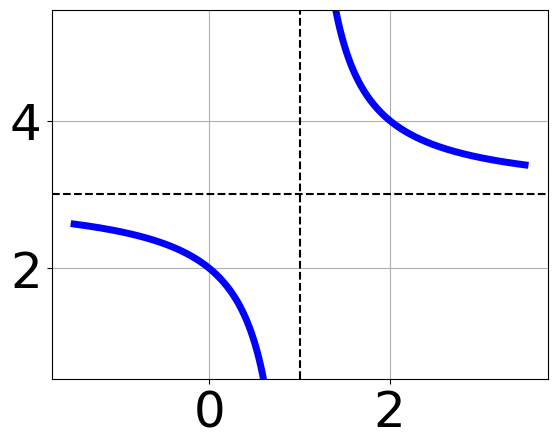
\includegraphics[width = 0.3\textwidth]{../Figures/rationalEquationToGraphDB.png}\end{multicols}\item None of the above.
\end{enumerate} }
\end{enumerate}

\end{document}